\IfFileExists{IEEEtran.cls}{\documentclass[conference]{IEEEtran}}{\documentclass[10pt,twocolumn]{article}}

\usepackage{amsmath,amssymb,amsfonts}
\usepackage{graphicx}
\usepackage{cite}
\usepackage{booktabs}
\usepackage{mathtools}
\usepackage{microtype}
\usepackage{placeins}
\usepackage{capt-of}
\usepackage{url}
\usepackage{xcolor}
\definecolor{RevisionGreen}{RGB}{0,105,40}
\definecolor{RevisionRed}{RGB}{185,32,32}
\newif\iftrackchanges
\newcommand{\added}[1]{\iftrackchanges{\color{RevisionGreen}#1}\else#1\fi}
\newcommand{\deleted}[1]{\iftrackchanges{\color{RevisionRed}#1}\fi}
\trackchangesfalse
\providecommand{\hl}[1]{#1}
\ifdefined\IEEEkeywords\else
\newenvironment{IEEEkeywords}{\par\noindent\textbf{Keywords: }}{\par}
\fi

\newcommand{\Nset}{\mathcal{N}}
\newcommand{\Dset}{\mathcal{D}}
\newcommand{\Cset}{\mathcal{C}}
\newcommand{\Vset}{\mathcal{V}}
\newcommand{\Mset}{\mathcal{M}}
\newcommand{\indicator}{\mathbf{1}}
\DeclareMathOperator*{\argmax}{arg\,max}

%\title{Priority-Aware SAGIN Support for Digital-Twin-Based Multi-Agent Robotic Coordination}
\title{Joint SAGIN Resource Allocation and Multi-Agent
Path Finding for Digital-Twin-Supported Remote
Robotic Applications}
\author{Irem Bor-Yaliniz, Arman Dogru, and Georges Kaddoum}

\begin{document}
\raggedbottom
\maketitle

\begin{abstract}
Remote multi-robot missions require both computation support and timely coordination information in environments where terrestrial infrastructure may be unavailable. This paper develops a space--air--ground integrated network (SAGIN) framework for digital-twin-supported multi-agent path finding. Drone-BS and ground-cloud processors produce robot-specific guidance and timestamped coordination states, using a low-Earth-orbit backhaul when cloud execution is selected. The frozen PANAMA action policy consumes local sensing and the received infrastructure caches at robot decision epochs. PANAMA priorities are also converted into bounded resource weights for computation allocation without modifying the priorities generated by the application. For fixed offloading decisions and radio rates, priority-aware processor allocation is obtained from KKT conditions, with a closed-form latency-only special case and explicit latency floors. To capture the application-level effect of delayed information, timestamped digital-twin states are represented by receiver caches and source-time age of information. A directed priority-inconsistency metric is then defined only for predicted vertex or edge conflicts inside PANAMA's square field of view. A conditional age bound characterizes recovery of the current PANAMA ordering. The resulting experiments measure the closed feedback loop from priorities to allocation, information freshness and subsequent multi-robot decisions.
\end{abstract}

\begin{IEEEkeywords}
space--air--ground integrated networks, digital twins, multi-agent path finding, age of information, task offloading, priority-aware resource allocation.
\end{IEEEkeywords}

\section{Introduction}
Teams of mobile robots are increasingly considered for search and rescue, inspection, defence, and mining missions. These environments may lack reliable terrestrial communication and computing infrastructure. A space--air--ground integrated network (SAGIN) can provide temporary access through a low-altitude Drone-BS and extend cloud connectivity through a low-Earth-orbit (LEO) satellite. The same architecture introduces transmission, propagation, and computation delays that affect both task completion and the freshness of the information used for robot coordination.

Digital twins provide an execution environment for computationally demanding coordination support. In PANAMA, asymmetric observations are created by exposing each robot to the communicated intentions of higher-priority robots within its field of view (FoV) \cite{dogru2025panama}. In the original formulation, these application quantities are immediately available to the observation constructor. Here, infrastructure processors generate guidance and coordination states from uploaded robot reports; the action network then consumes received states alongside local sensing. A robot may compare stale versions of its own priority and a peer priority, which can reverse the intended yielding relation. Conventional SAGIN offloading models do not capture this consequence because they optimize communication and computation metrics without representing the coordination decision that consumes the delivered information. Serializing the action network itself behind a remote observation--action exchange would require a separate execution and timing model.

This paper addresses that gap through the following contributions:
\begin{itemize}
    \item A SAGIN architecture offloads digital-twin coordination support to Drone-BS or ground-cloud processors and delivers timestamped guidance and coordination states to the PANAMA action policy.
    \item PANAMA priorities are mapped to bounded resource weights. For fixed offloading decisions and radio rates, Drone-BS and cloud CPU allocations are obtained, with a closed-form latency-only special case and a dynamic-energy KKT solution.
    \item A receiver-dependent priority-inconsistency metric is introduced. The metric is restricted to predicted vertex and edge conflicts inside PANAMA's square FoV and is explicitly coupled to source-time age of information (AoI).
    \item A communication-to-coordination relationship is established through an exact AoI condition for a current priority ordering and conservative bounds on stale decision epochs and additional waiting time.
\end{itemize}

The remainder of the paper is organized as follows. Section~II presents the SAGIN, task, and information models. Section~III formulates priority-aware resource allocation and derives its main latency properties. Section~IV integrates delayed digital-twin information with PANAMA and develops the inconsistency analysis. Section~V distinguishes frozen-policy evaluation from the learning-transport extension. Section~VI presents simulation assumptions and results, and Section~VII concludes the paper.

\section{System Model}
\subsection{SAGIN and Task Model}
Let $\Nset=\{1,\ldots,N\}$ denote the robots. Robot $i$ generates a task
\begin{equation}
    \mathcal{T}_i=\{s_i,c_i\},
\end{equation}
where $s_i$ is the logical input size and $c_i$ is the number of CPU cycles per input bit. The total required work is $C_i=s_ic_i$. The mission study imposes no hard task deadline; $\tau_i$ is retained only in the separate analytical feasibility discussion and solver validation tests. A binary variable $x_i$ selects Drone-BS processing when $x_i=1$ and ground-cloud processing through the LEO backhaul when $x_i=0$. The assigned computation rates are $f_{D,i}$ and $f_{C,i}$.


\begin{figure*}[t]
    \centering
    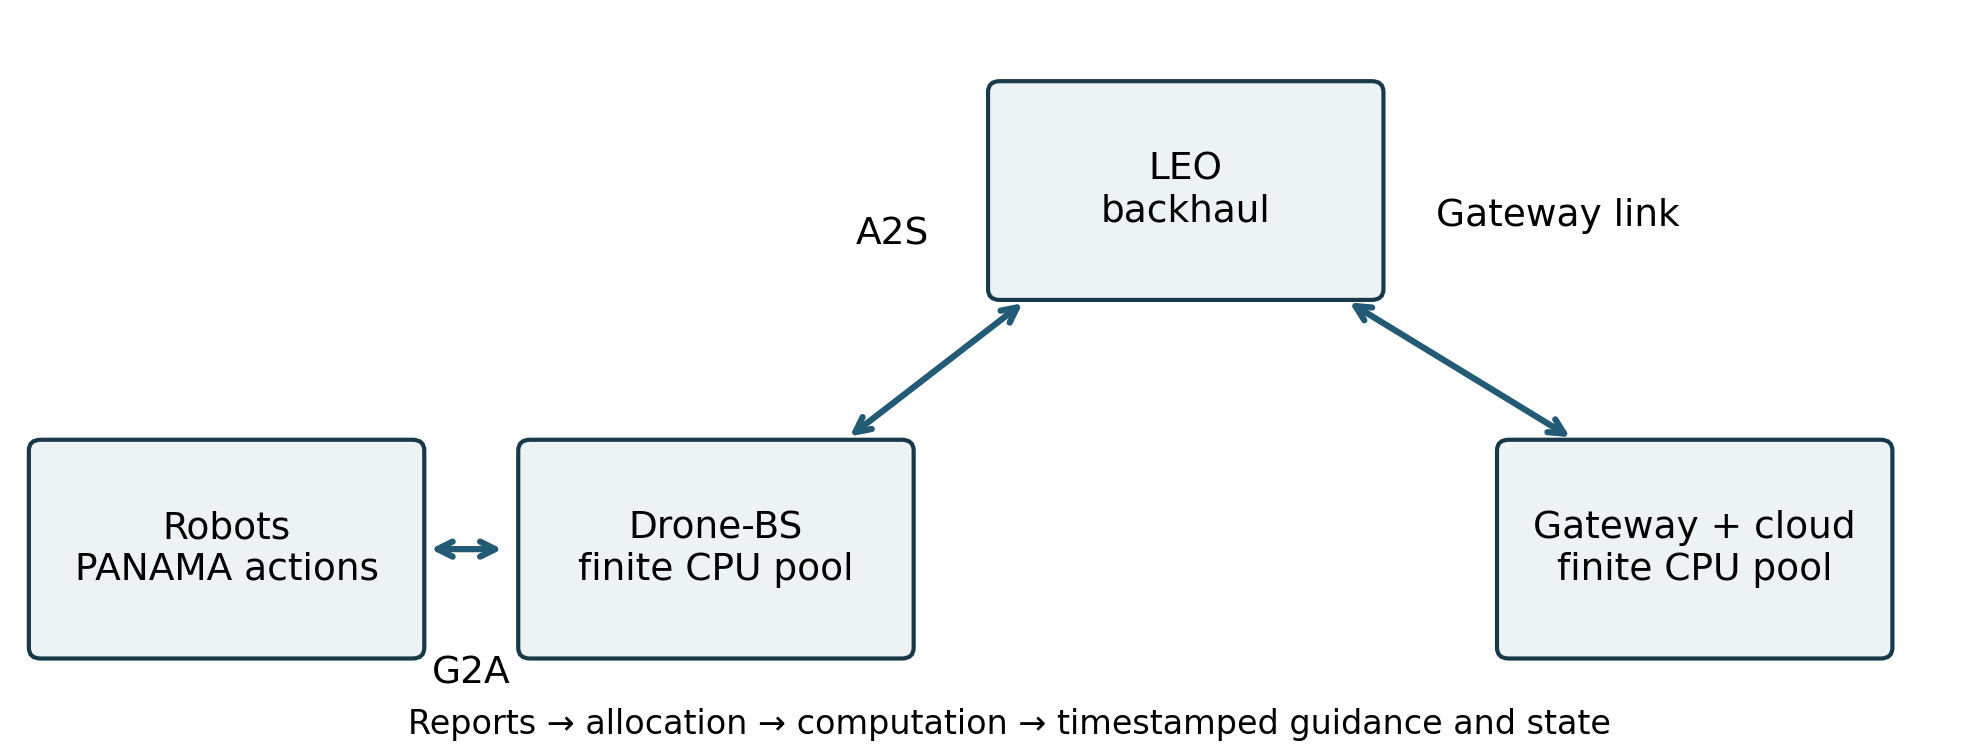
\includegraphics[width=.85\textwidth]{figures/system_model.png}
    \caption{Offloaded digital-twin coordination support and PANAMA action decisions using received caches. Cloud jobs traverse the complete LEO and gateway route.}
    \label{fig:system}
\end{figure*}

\subsection{Air-to-Ground Access}
The air-to-ground model follows the probabilistic line-of-sight model in \cite{boryaliniz2019spatial}. Let $h_D$ be the Drone-BS altitude and let $r_i$ be the horizontal distance between robot $i$ and the Drone-BS. The probability of a line-of-sight connection is
\begin{equation}
    P_{\mathrm{LoS}}(h_D,r_i)
    =
    \frac{1}{1+a\exp\!\left[-b\left(\frac{180}{\pi}\tan^{-1}\!\left(\frac{h_D}{r_i}\right)-a\right)\right]},
    \label{eq:los_probability}
\end{equation}
where $a$ and $b$ depend on the deployment environment. The average path loss in dB is
\begin{equation}
    L_i^{\mathrm{G2A}}
    =
    20\log_{10}\!\left(\sqrt{h_D^2+r_i^2}\right)
    +z_1P_{\mathrm{LoS}}(h_D,r_i)+z_2,
    \label{eq:g2a_pathloss}
\end{equation}
where
\begin{equation}
    z_1=\eta_{\mathrm{LoS}}-\eta_{\mathrm{NLoS}},\qquad
    z_2=20\log_{10}\!\left(\frac{4\pi f_c}{c_0}\right)+\eta_{\mathrm{NLoS}}.
\end{equation}
Here, $f_c$ is the carrier frequency, $c_0$ is the speed of light, and $\eta_{\mathrm{LoS}}$ and $\eta_{\mathrm{NLoS}}$ are the excessive losses for the two propagation states. For bandwidth $B_i^{\mathrm{G2A}}$ and transmit power $P_i$, the uplink rate is
\begin{equation}
    R_i^{\mathrm{G2A}}
    =B_i^{\mathrm{G2A}}
    \log_2\!\left(1+
    \frac{P_i10^{-L_i^{\mathrm{G2A}}/10}}
    {N_0B_i^{\mathrm{G2A}}}\right),
    \label{eq:g2a_rate}
\end{equation}
where $N_0$ is the noise power spectral density.

\subsection{Air-to-Space Backhaul}
Let $\bar d_{\mathrm{sat}}$ be the average Drone-BS-to-satellite distance during an association interval. The air-to-space path loss is
\begin{equation}
    L^{\mathrm{A2S}}
    =20\log_{10}\!\left(\frac{4\pi f_{\mathrm{sat}}\bar d_{\mathrm{sat}}}{c_0}\right)+\xi_{\mathrm{atm}},
\end{equation}
where $f_{\mathrm{sat}}$ is the carrier frequency and $\xi_{\mathrm{atm}}$ is atmospheric attenuation. With bandwidth $B_i^{\mathrm{A2S}}$, Drone-BS transmit power $P_D$, and channel gain $\lVert g_i\rVert^2$, the rate is
\begin{equation}
    R_i^{\mathrm{A2S}}
    =B_i^{\mathrm{A2S}}
    \log_2\!\left(1+
    \frac{P_D\lVert g_i\rVert^2 10^{-L^{\mathrm{A2S}}/10}}
    {N_0B_i^{\mathrm{A2S}}}\right).
\end{equation}

\subsection{Task Latency}
The latency for Drone-BS execution is
\begin{equation}
    T_{i,D}
    =
    \frac{s_i}{R_i^{\mathrm{G2A}}}
    +
    \frac{C_i}{f_{D,i}}.
    \label{eq:drone_latency}
\end{equation}
where $f_{D,i}$ is the Drone-AP computation capacity allocated to $\mathcal{T}_i$ in terms of CPU cycles per second.
For cloud execution,
\begin{equation}
    T_{i,C}
    =
    \frac{s_i}{R_i^{\mathrm{G2A}}}
    +
    \frac{s_i}{R_i^{\mathrm{A2S}}}
    +T_{\mathrm{prop}}
    +
    \frac{C_i}{f_{C,i}},
    \label{eq:cloud_latency}
\end{equation}
where $T_{\mathrm{prop}}=2[(\bar d_{\mathrm{sat}}+\bar d_{\mathrm{gw}})/c_0+d_{\mathrm{ground}}]$ includes the outbound and return space legs and the terrestrial contribution. The approximation $2\bar d_{\mathrm{sat}}/c_0$ applies only if gateway and terrestrial propagation are omitted. The task latency is $T_i=x_iT_{i,D}+(1-x_i)T_{i,C}$. The analytical expression neglects small result serialization; the simulator retains actual response serialization, contention, guard intervals, interruptions and changes in processor sharing.

\subsection{Energy Model}
The transmission energy expended by robot $i$ is
\begin{equation}
E_i^{\mathrm{tx}}=P_i\frac{s_i}{R_i^{\mathrm{G2A}}}.
\end{equation}
With fixed powers and rates, this robot-upload term is constant within a scheduling snapshot. It is excluded from the optimization objective and retained in physical energy measurements. The dynamic-voltage-and-frequency-scaling model gives the Drone-BS energy
\begin{equation}
E_{D,i}=x_i\kappa_D f_{D,i}^2C_i+(1-x_i)P_D\frac{s_i}{R_i^{\mathrm{A2S}}},
\end{equation}
where $\kappa_D$ is an assumed switched-capacitance coefficient. Static processor power, cooling, propulsion, optical pointing, cloud electricity and downlink transmitter energy are outside this model; the reported energy is explicitly the modeled robot upload, drone backhaul and drone dynamic CPU energy.
\begin{figure*}[t]
    \centering
    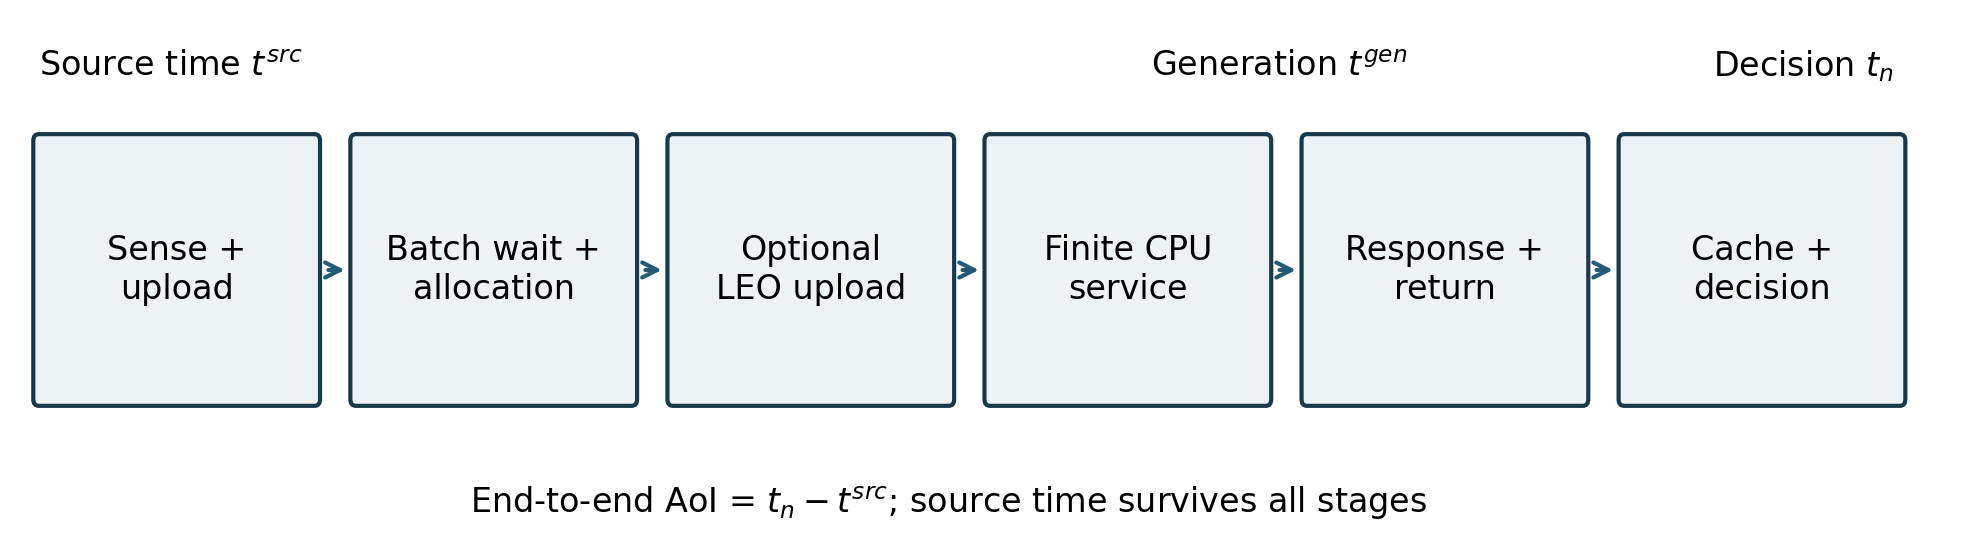
\includegraphics[width=.85\textwidth]{figures/timing.png}
    \caption{System model and delay sources.}
    \label{fig:delay}
\end{figure*}

\subsection{End-to-End Information Freshness} \label{subsec:end_to_end_information_freshness} Digital-twin coordination support executes at the selected Drone-BS or ground-cloud processor. The information delivered to a physical robot may already be stale when the corresponding digital-twin message is generated. This staleness originates from the robot-to-digital-twin uplink, waiting and processing at the digital-twin layer, and the subsequent digital-twin-to-robot downlink as shown in Fig.~\ref{fig:delay}. Let \begin{equation} U_j(k) = \left( q_j(k), g_j(k), \mathcal{L}_j(k) \right) \end{equation} denote the \(k\)th physical-state report of robot \(j\), where \(q_j(k)\) is its sensed position, \(g_j(k)\) is its goal status, and \(\mathcal{L}_j(k)\) contains any additional information required by the digital twin, such as locally sensed information and operational state. The report is sampled at time \(t_{j,k}^{\mathrm{sense}}\) and reaches the digital twin at
\begin{equation} t_{j,k}^{\mathrm{DT-arr}} = t_{j,k}^{\mathrm{sense}} + \delta_{j,k}^{\mathrm{UL}}, \label{eq:dt_uplink_arrival}
\end{equation}
where \(\delta_{j,k}^{\mathrm{UL}}\) is the corresponding uplink delay. The digital twin uses the received physical-state reports to generate the coordination state
\begin{equation} S_j(n) = \left( I_j(n), \rho_j(n), g_j(n) \right), \label{eq:coordination_state}
\end{equation}
where \(I_j(n)\) is the intended path segment and \(\rho_j(n)\) is the priority generated by PANAMA. Each downlink message \(m\) contains a payload \(\psi_m\), a generation time \(t_m^{\mathrm{gen}}\), a source-information time \(t_m^{\mathrm{src}}\), and a sequence number \(\nu_m\). The source time is not the time at which the digital twin creates the message. Instead, it records the physical sensing time of the dynamic information used to generate the payload. Let \(\mathcal{D}_m\) denote the set of dynamic physical reports used to generate message \(m\). The source-information time is defined as \begin{equation} t_m^{\mathrm{src}} = \min_{\ell\in\mathcal{D}_m} t_{\ell}^{\mathrm{sense}}. \label{eq:message_provenance_time} \end{equation} Thus, \(t_m^{\mathrm{src}}\leq t_m^{\mathrm{gen}}\), and the difference \begin{equation} A_m^{\mathrm{pre}} = t_m^{\mathrm{gen}} - t_m^{\mathrm{src}} \label{eq:pregeneration_age} \end{equation} captures the age accumulated before message generation, including uplink transmission, digital-twin waiting, and digital-twin processing. The message arrives at its receiver at \begin{equation} t_m^{\mathrm{arr}} = t_m^{\mathrm{gen}} + \delta_m^{\mathrm{DL}}, \label{eq:downlink_arrival} \end{equation} where \(\delta_m^{\mathrm{DL}}\) is the delivery delay from the digital-twin layer to the physical robot. Let \(\mathcal{M}_i^\sigma(t)\) denote the messages of stream \(\sigma\) received by robot \(i\) by time \(t\). At decision epoch \(n\), robot \(i\) accepts \begin{equation} m_i^{\sigma,*}(n) = \arg\max_{m\in\mathcal{M}_i^\sigma(t_n)} \left( t_m^{\mathrm{gen}}, \nu_m \right) \label{eq:accepted_message} \end{equation} under lexicographic ordering. The end-to-end AoI of the accepted stream is \begin{equation} A_i^\sigma(n) = t_n - t_{m_i^{\sigma,*}(n)}^{\mathrm{src}}. \label{eq:end_to_end_aoi} \end{equation} It can be decomposed as \begin{align} A_i^\sigma(n) = &\underbrace{ t_{m_i^{\sigma,*}(n)}^{\mathrm{gen}} - t_{m_i^{\sigma,*}(n)}^{\mathrm{src}} }_{\text{uplink, waiting, and DT processing}} \nonumber\\ &+ \underbrace{ t_n - t_{m_i^{\sigma,*}(n)}^{\mathrm{gen}} }_{\text{downlink delivery and cache residence}}. \label{eq:aoi_decomposition} \end{align} The second component may be reported separately as the post-generation age \begin{equation} A_{i,\mathrm{post}}^\sigma(n) = t_n - t_{m_i^{\sigma,*}(n)}^{\mathrm{gen}}. \label{eq:postgeneration_age} \end{equation} The primary freshness measure in this work remains the end-to-end AoI in \eqref{eq:end_to_end_aoi}, because it includes the complete physical-robot-to-digital-twin-to-robot information path.

\section{Priority-Aware Resource Allocation}
PANAMA priorities are application outputs rather than optimization variables.
In the retained implementation, let $M$ be the number of grid cells and let
$\ell_i$ be the shortest remaining path length. The application uses
\begin{equation}
\rho_i=\begin{cases}
M+10^{-6}i,&\text{completed},\\
\min\{\ell_i,M-1\}+10^{-6}i,&\text{active},
\end{cases}
\end{equation}
where completion means first reaching the goal and an unreachable active path is
assigned $M-1$ before the robot-ID offset.
Smaller values have higher application priority. For the studied populations this
keeps every completed robot strictly below every active robot, including an
unreachable one. The infrastructure applies this convention to available reports.
To let the infrastructure respond to those priorities, define the bounded resource weight
\begin{equation}
    \pi_i(n)=\pi_{\min}+(\pi_{\max}-\pi_{\min})
    \frac{\rho_{\max}-\rho_i(n)}{\rho_{\max}-\rho_{\min}},
    \label{eq:priority_weight}
\end{equation}
where $0<\pi_{\min}\leq\pi_i(n)\leq\pi_{\max}$. The transformation preserves PANAMA's order but does not modify its priorities. The ratio $\pi_{\max}/\pi_{\min}$ controls the maximum resource differentiation and prevents a low-priority task from receiving zero weight.
The extrema are calculated over active reports available to the infrastructure. Equal active priorities receive $\pi_{\max}$, while completed agents receive $\pi_{\min}$. Completed-agent application priorities remain below all active agents in the smaller-is-higher ordering, including an unreachable active path; deterministic robot-ID offsets break ties.

For one scheduling interval, consider
\begin{subequations}\label{prob:joint}
\begin{align}
\min_{\boldsymbol{x},\boldsymbol{f}_D,\boldsymbol{f}_C}\quad
&\sum_{i=1}^{N}\left(\omega_2\pi_iT_i+\omega_3E_{D,i}\right) \\
\mathrm{s.t.}\quad
%&0\leq P_i\leq P_i^{\max}, &&i\in\Nset,\\
&\sum_{i=1}^{N}x_if_{D,i}\leq F_D^{\max},\\
&\sum_{i=1}^{N}(1-x_i)f_{C,i}\leq F_C^{\max},\\
&f_{D,i},f_{C,i}\geq0,\quad x_i\in\{0,1\}, &&i\in\Nset.
\end{align}
\end{subequations}
Additional platform energy requires calibrated propulsion and static-power models. The formulation in \eqref{prob:joint} is a mixed-integer nonlinear program.

\subsection{Closed-Form Computation Allocation}
The square-root expressions below solve the latency-oriented special case, with zero drone CPU-energy penalty. They must not be substituted unchanged into the full latency-plus-DVFS objective. For that objective, with fixed binary assignments, the active drone rates satisfy
\begin{equation}
 -\frac{\omega_2\pi_iC_i}{f_{D,i}^2}
 +2\omega_3\kappa_D C_i f_{D,i}+\lambda_D=0,
 \quad\lambda_D\geq0,
 \label{eq:dvfs_kkt}
\end{equation}
with complementary slackness on the total CPU capacity. A scalar multiplier solve gives the unique positive rates for positive workloads and latency weights; capacity can remain idle. Cloud computation retains the latency-only square-root rule because cloud electricity is not included in the objective.

For fixed offloading decisions and radio rates, define $\Dset=\{i:x_i=1\}$ and $\Cset=\{i:x_i=0\}$. The latency-oriented Drone-BS subproblem is
\begin{equation}
    \min_{\{f_{D,i}>0\}}
    \sum_{i\in\Dset}\pi_i\frac{C_i}{f_{D,i}}
    \quad\mathrm{s.t.}\quad
    \sum_{i\in\Dset}f_{D,i}\leq F_D^{\max}.
\end{equation}
Its KKT conditions give
\begin{equation}
    f_{D,i}^{*}
    =F_D^{\max}
    \frac{\sqrt{\pi_iC_i}}
    {\sum_{j\in\Dset}\sqrt{\pi_jC_j}},
    \label{eq:optimal_drone_cpu}
\end{equation}
with the analogous cloud allocation
\begin{equation}
    f_{C,i}^{*}
    =F_C^{\max}
    \frac{\sqrt{\pi_iC_i}}
    {\sum_{j\in\Cset}\sqrt{\pi_jC_j}}.
\end{equation}
The resulting Drone-BS latency is
\begin{equation}
    T_{i,D}^{*}
    =d_{i,D}+\frac{C_i}{F_D^{\max}}
    +\frac{\sqrt{C_i}}{F_D^{\max}\sqrt{\pi_i}}
    \sum_{\substack{j\in\Dset\\j\neq i}}\sqrt{\pi_jC_j},
    \label{eq:priority_delay}
\end{equation}
where $d_{i,D}=s_i/R_i^{\mathrm{G2A}}$. Holding competing weights fixed, $\partial T_{i,D}^{*}/\partial\pi_i\leq0$. The minimum attainable latency under fixed rate and offloading is
\begin{equation}
    \lim_{\pi_i\rightarrow\infty}T_{i,D}^{*}
    =d_{i,D}+\frac{C_i}{F_D^{\max}}.
\end{equation}
The bounded mapping in \eqref{eq:priority_weight} excludes the starvation limit $\pi_i\rightarrow0$. For a fixed Drone-BS task set, all deadlines are feasible if and only if
\begin{equation}
    \tau_i>d_{i,D},\quad i\in\Dset,
    \qquad
    \sum_{i\in\Dset}\frac{C_i}{\tau_i-d_{i,D}}\leq F_D^{\max}.
    \label{eq:deadline_feasibility}
\end{equation}
The same result holds for the cloud after replacing $d_{i,D}$ and $F_D^{\max}$ with $d_{i,C}=s_i/R_i^{\mathrm{G2A}}+s_i/R_i^{\mathrm{A2S}}+T_{\mathrm{prop}}$ and $F_C^{\max}$. Equations \eqref{eq:optimal_drone_cpu}--\eqref{eq:deadline_feasibility} characterize computation sharing.
\subsection{Validated Binary Execution and Scheduling Relaxation}
Each fixed-input snapshot is solved by enumerating the binary decisions for its at most eight new tasks. Previous unfinished tasks retain their assignments and remaining work in the capacity constraints. Each assignment uses \eqref{eq:dvfs_kkt} and the cloud square-root rule; the least-cost assignment is executed. Processor shares are updated on arrivals and completions, so the snapshot prediction is recorded separately from observed latency.
The numerical implementation scales perspective epigraphs by their workload/objective coefficients, removes the unused cones for unavailable routes, and recovers feasible CPU shares by minimizing the same fixed-$x$ convex subproblem. Clarabel targets $10^{-8}$ tolerances, with a recorded cold numerical retry at $10^{-7}$ if needed; accepted capacity/conic residuals and recovered-objective agreement must still satisfy $10^{-6}$. A numerical retry never changes the objective or execution policy.

An independently reported continuous scheduling bound uses $x_i\in[0,1]$ and
\begin{equation}
 a_i=x_i f_{D,i}/F_D^{\max},\qquad
 b_i=(1-x_i)f_{C,i}/F_C^{\max}.
\end{equation}
Its latency and drone energy are
\begin{align}
 T_i={}&d_{i,D}+(1-x_i)(d_{i,C}-d_{i,D})\nonumber\\
 &+\frac{C_i}{F_D^{\max}}\frac{x_i^2}{a_i}
 +\frac{C_i}{F_C^{\max}}\frac{(1-x_i)^2}{b_i},\\
 E_{D,i}={}&\kappa_D C_i(F_D^{\max})^2\frac{a_i^2}{x_i}
 +(1-x_i)P_Ds_i/R_i^{\mathrm{A2S}},
\end{align}
subject to $\sum_i a_i\leq1$, $\sum_i b_i\leq1$, $0\leq a_i\leq x_i\leq1$, and $0\leq b_i\leq1-x_i$. The closed quadratic-over-linear perspectives are represented by second-order cones, including the zero-work endpoints. CVXPY/Clarabel certifies convexity. Fractional $x_i$ is a scheduling relaxation, not simultaneous execution of physically split jobs. We check the relaxed objective against the exact binary optimum and preserve failed snapshots without substituting another policy. Optimality applies to the scheduling snapshot, not the evolving mission.


\section{Delayed PANAMA Coordination}
\subsection{End-to-End Priority Inconsistency}
\label{subsec:end_to_end_priority_inconsistency}

Communication delay can affect the PANAMA ordering at two stages. First, delayed physical-state reports may cause the digital twin to calculate priorities from stale robot states. Second, delayed delivery of the resulting coordination states may cause a physical robot to apply an outdated digital-twin ordering.

Let
\begin{equation}
    \rho_j^{\mathrm{phys}}(n)
\end{equation}
denote the priority that PANAMA would generate using the current physical state of robot \(j\), and let
\begin{equation}
    \rho_j^{\mathrm{DT}}(n)
\end{equation}
denote the priority actually generated by the digital twin using the latest physical-state reports available to it.

The current physical ordering is
\begin{equation}
    \chi_{j\prec i}^{\mathrm{phys}}(n)
    =
    \mathbf{1}
    \left\{
        \rho_j^{\mathrm{phys}}(n)
        <
        \rho_i^{\mathrm{phys}}(n)
    \right\}.
    \label{eq:physical_priority_relation}
\end{equation}

The digital-twin ordering is
\begin{equation}
    \chi_{j\prec i}^{\mathrm{DT}}(n)
    =
    \mathbf{1}
    \left\{
        \rho_j^{\mathrm{DT}}(n)
        <
        \rho_i^{\mathrm{DT}}(n)
    \right\}.
    \label{eq:dt_priority_relation}
\end{equation}

The ordering applied by robot \(i\) is
\begin{equation}
    \widehat{\chi}_{j\prec i}^{(i)}(n)
    =
    \mathbf{1}
    \left\{
        \widehat{\rho}_{j\rightarrow i}(n)
        <
        \widehat{\rho}_{i\rightarrow i}(n)
    \right\}.
    \label{eq:perceived_priority_relation}
\end{equation}

The uplink-induced ordering error is
\begin{equation}
    \Xi_{j\rightarrow i}^{\mathrm{UL}}(n)
    =
    \left|
        \chi_{j\prec i}^{\mathrm{DT}}(n)
        -
        \chi_{j\prec i}^{\mathrm{phys}}(n)
    \right|.
    \label{eq:uplink_ordering_error}
\end{equation}

The post-generation delivery error is
\begin{equation}
    \Xi_{j\rightarrow i}^{\mathrm{DL}}(n)
    =
    \left|
        \widehat{\chi}_{j\prec i}^{(i)}(n)
        -
        \chi_{j\prec i}^{\mathrm{DT}}(n)
    \right|.
    \label{eq:downlink_ordering_error}
\end{equation}

The end-to-end ordering error is
\begin{equation}
    \Xi_{j\rightarrow i}^{\mathrm{E2E}}(n)
    =
    \left|
        \widehat{\chi}_{j\prec i}^{(i)}(n)
        -
        \chi_{j\prec i}^{\mathrm{phys}}(n)
    \right|.
    \label{eq:end_to_end_ordering_error}
\end{equation}

These metrics satisfy
\begin{equation}
    \Xi_{j\rightarrow i}^{\mathrm{E2E}}(n)
    \leq
    \Xi_{j\rightarrow i}^{\mathrm{UL}}(n)
    +
    \Xi_{j\rightarrow i}^{\mathrm{DL}}(n).
    \label{eq:ordering_error_decomposition}
\end{equation}

Using the FoV relevance indicator \(\zeta_{j\rightarrow i}(n)\), the coordination-relevant end-to-end inconsistency is
\begin{equation}
    \widetilde{\Xi}_{j\rightarrow i}^{\mathrm{E2E}}(n)
    =
    \zeta_{j\rightarrow i}(n)
    \Xi_{j\rightarrow i}^{\mathrm{E2E}}(n).
    \label{eq:fov_e2e_inconsistency}
\end{equation}

The corresponding AoI-weighted metric is
\begin{equation}
    \widetilde{\Xi}_{j\rightarrow i}^{A,\mathrm{E2E}}(n)
    =
    \widetilde{\Xi}_{j\rightarrow i}^{\mathrm{E2E}}(n)
    \frac{
        \max
        \left\{
            A_i^{S_j}(n),
            A_i^{S_i}(n)
        \right\}
    }{
        A_{\mathrm{ref}}
    }.
    \label{eq:aoi_weighted_e2e_inconsistency}
\end{equation}

The AoI values in \eqref{eq:aoi_weighted_e2e_inconsistency} are measured from the robot's information generation times supporting the accepted digital-twin coordination states. They therefore include uplink delay, digital-twin waiting and processing, downlink delay, and cache residence.


\section{Event-Driven Learning and Evaluation}
The resource-allocation results freeze the previously qualified clean policy; no learner updates change its weights between allocation conditions. The closed loop repeatedly executes PANAMA inference at robot decision epochs, calculates reported application priorities, optimizes resources, delivers completed guidance/states and executes PANAMA again using the resulting observations. The following learning-transport equations describe a possible extension; learning-delay arms are not measured in this study.
After action $n$, robot $i$ forms
\begin{equation}
    \zeta_i(n)=\big(\widehat o_i(n),a_i(n),r_i(n+1),
    \widehat o_i(n+1),\mathrm{done}_i(n+1)\big),
\end{equation}
where $\mathrm{done}_i(n+1)\in\{0,1\}$ is the terminal flag. The transition arrives at the cloud learner at $t_i^E(n)=t_{n+1}+\delta_i^E(n)$. For a sampled transition $\zeta=(o,a,r,o',\mathrm{done})$, the Double DQN target is
\begin{equation}
    y_\zeta=r+\gamma(1-\mathrm{done})Q_{\theta^-}
    \left(o',\argmax_{a'}Q_\theta(o',a')\right).
\end{equation}
After learner update $\ell$, snapshot $\Theta_\ell$ is released at $t_\ell^{\mathrm{rel}}$ and reaches robot $i$ at $t_i^W(\ell)=t_\ell^{\mathrm{rel}}+\delta_i^W(\ell)$. Robot $i$ installs the newest complete snapshot available before $t_n$. Timestamp and version checks prevent rollback.

Mission experiments use the fixed policy and explicitly simulate guidance and coordination-state delivery. Equal resource weights, static priorities, AoI-only weights and current PANAMA-priority weights are compared using task latency, energy, mission completion, censored duration, sum of path costs, stationary steps, $\Xi^{\mathrm{FoV}}$ and source-time AoI. No mission task deadline is imposed. Future learning-delay experiments could compare immediate delivery, delayed experience uploads, delayed model delivery and both delays, adding replay age and model-version lag as outcomes.

\section{Simulations and Results}
\subsection{Reproducible Settings and Timing}
The experiments use the fixed MovingAI \texttt{random-32-32-10} map, with 32 by 32 cells and one metre per cell. Robot actions are the four cardinal moves or waiting; each control cycle is one second. A square FoV of radius seven cells and five future intention cells are retained. The UAV starts at the map centre and its analytical coverage-optimal reference altitude. Its three-dimensional motion is limited to one metre per control cycle toward the maximum-coverage target computed from successfully received position reports, with a 20 m minimum altitude. No fresh simulator position is supplied to the allocation or placement controllers.

The clean frozen PANAMA checkpoint qualified on 200 episodes at each population: success rates were 97\%, 96\%, 95.5\%, and 95\% for 2, 4, 6, and 8 robots. Evaluation uses 50 separate held-out cases per population and a 250-step cap. All treatments share policy weights, starts, goals, seeds and orbital offsets. Hashes identify the checkpoint, map, case bank, channel archive and source code. Map compatibility permits exact LF/CRLF conversion only.

The 100 ms control observation budget determines which cached information is available before an action. It is not a hard task deadline. One logical coordination task is generated per robot per cycle after the initial fresh briefing. The task size and CPU demand below are simulation assumptions, not profiled neural-inference workloads or measured processor performance. Whole tasks retain their execution site once assigned; the finite processors account for existing work and recompute priority-aware sharing on arrivals and completions. CPU service is work-conserving in the latency-only case and may intentionally idle under the DVFS objective. Actual dynamic CPU energy integrates $\kappa_D f_i(t)^3$ over service.

\begin{table}[t]
\centering\caption{Nominal access, computation and timing assumptions.}
\label{tab:nominal_parameters}\scriptsize
\begin{tabular}{@{}p{0.58\columnwidth}p{0.35\columnwidth}@{}}
\toprule Parameter & Value\\\midrule
G2A carrier; per-link bandwidth & 2.5 GHz; 20 MHz\\
Urban $a,b$; excess LoS/NLoS losses & 9.61, 0.16; 1/20 dB\\
Thermal PSD; receiver noise figure & $-174$ dBm/Hz; 7 dB\\
Effective receiver PSD & $-167$ dBm/Hz\\
Robot conducted uplink power & 0.2 W\\
Access uplink/downlink service ceilings & 50/50 Mbit/s\\
Task logical input; cycles per bit & $10^5$ bits; $10^3$\\
Drone/cloud CPU capacity & $10^9/10^{10}$ cycles/s\\
Drone dynamic CPU coefficient & $\kappa_D=10^{-28}$\\
Resource weights; completed-agent weight & $[1,4]$; 1\\
Latency/energy coefficients & $1$ s$^{-1}$/$1$ J$^{-1}$\\
Control cycle; observation budget & 1 s; 0.1 s\\
Maximum fragment; wire overhead & 65,536 B; 48 B/fragment\\
Hard mission-task deadline & None\\\bottomrule
\end{tabular}
\end{table}

\subsection{Channels, LEO Geometry and Propagation}
G2A uses the probabilistic urban LoS mean path loss in \eqref{eq:g2a_pathloss}; no instantaneous small-scale fading is drawn. The thermal PSD and receiver noise figure are applied once, so the effective PSD equals $-167$ dBm/Hz. The rate in \eqref{eq:g2a_rate} is additionally capped by the configured shared access-service capacity. Access is time-shared with round-robin queue service; the bandwidth is not multiplied by the number of simultaneous robots. Upload input bits and actual serialized wire bits are recorded separately. To retain checkpoint compatibility, the policy's third observation channel remains PANAMA's normalized coverage-margin proxy. That proxy is distinct from the physical RF SNR used to calculate the actual access rate and is not reported as a calibrated SNR measurement.

The orbital archive contains six hours of one-second SGP4/Skyfield geometry replayed at its archived epoch, 31 August 2026. The reference site is $(46.2^{\circ},-74.6^{\circ})$ at 440 m elevation; the assumed gateway is $(45.3^{\circ},-74.6^{\circ})$ at 300 m. These coordinates are model inputs, not a measured provider gateway. The highest visible satellite is selected at 15 s scheduling boundaries, with a $25^{\circ}$ terminal and $10^{\circ}$ gateway elevation mask. Original 50 ms attachment/reconfiguration interruptions are retained. Frames are 20 ms with a 5\% service guard.

To implement the association-average assumption, terminal and gateway ranges and statistical attenuation in dB are averaged within each association/scheduling interval. Free-space loss, SNR and Shannon rates are then recomputed from those mean inputs; arithmetic means of rates are not substituted. ITU-Rpy 0.4.0 provides the archived P.618 statistical atmospheric predictions \cite{iturP618} at a fixed 1\% exceedance quantile. This quantile is not a sampled weather process. No provider modulation or beam-scheduler reconstruction is claimed. Small within-map UAV displacement is neglected in the orbital geometry; the conservative round-trip propagation error bound is below $0.7$ microseconds, while G2A uses the actual UAV placement.

\begin{table}[t]
\centering\caption{Backhaul engineering assumptions and full-route delays.}
\label{tab:backhaul_parameters}\scriptsize
\begin{tabular}{@{}p{0.58\columnwidth}p{0.35\columnwidth}@{}}
\toprule Parameter & Value\\\midrule
Uplink/downlink carrier & 14.25/11.7 GHz\\
Uplink/downlink bandwidth & 20/100 MHz\\
Drone conducted satellite-uplink power & 2 W\\
Terminal EIRP; implied uplink antenna gain & 35 dBW; 31.99 dBi\\
Satellite receive $G/T$ & $-5$ dB/K\\
Satellite EIRP; terminal receive $G/T$ & 30 dBW; 5 dB/K\\
Implementation loss; Shannon efficiency & 3 dB; 0.5\\
Atmospheric antenna diameter; exceedance & 0.3 m; 1\%\\
Nominal backhaul uplink/downlink ceilings & 10/50 Mbit/s\\
One-way ground-network propagation & 10 ms\\
Association-average full-route RTT & 24.92--29.60 ms\\\bottomrule
\end{tabular}
\end{table}

The full route is robot--UAV--LEO--gateway--ground cloud and its reverse, with no inter-satellite hop. Each direction is limited by both its terminal and gateway link budgets. Conducted transmitter power, rather than EIRP, determines transmission energy. Propagation includes one outbound and one return contribution; fragmentation does not multiply propagation by the number of fragments. Actual response serialization is simulated even though it is omitted from the analytical latency expression. Solver wall time is measured separately from logical task CPU time.

\subsection{Validation, Baselines and Metrics}
Six predictable sanity cases cover large satellite delay, fast cloud/slow drone, unavailable backhaul, unavailable drone CPU, fixed-route priority differentiation and a DVFS optimum with idle CPU. Every expected assignment is checked using an independent primal CVXPY formulation and exhaustive enumeration. The earlier supplied four-robot MATLAB validation inputs are also preserved, including the original infinite deadlines and the separate Case E feasibility test; execution here uses the approved CVXPY equivalent.

The primary grid combines uplink and common CPU multipliers $\{0.25,1,4\}$ under equal resource weights, episode-initial static priorities, AoI-only weights and current PANAMA-priority weights, with one fresh-coordination reference. Separate sensitivity conditions vary drone CPU, cloud CPU, downlink, logical input and cycles/bit by 0.25 and 4, the weight ratio by 1 and 16 (baseline 4), and the energy coefficient by 0, 0.1 and 10 (latency coefficient 1). There are 97 total conditions and 19,400 paired episodes. The ideal fresh reference has instantaneous coordination and no modeled support-task energy; its energy is not a hardware benchmark.

Task outcomes include observed and snapshot-predicted latency, prediction error, the 95th latency percentile, unfinished-task counts, stage service times, and modeled energy by transmitter and processor. Mission outcomes include completion, capped mission duration, successful makespan, sum of time-to-first-arrival costs, stationary steps (including blocked moves), and collision attempts. Unfinished missions remain censored at 250 steps; PAR-2 assigns them 500. Directed inconsistency is recorded with UL/DL/E2E decomposition, square-FoV relevance, source-time AoI and raw numerator/denominator counts. Mean per-episode inconsistency and pooled relevant-pair ratios are labelled separately. A zero relevance denominator gives zero.

Each comparison uses the same held-out case in both conditions. We report paired mean differences and seeded 2,000-resample 95\% bootstrap intervals, with the number of usable pairs for metrics affected by censoring. The intervals are pointwise across the sensitivity grid and are not family-wise multiple-comparison guarantees. Conditional successful makespans are secondary to completion and PAR-2. Snapshot optimality and a lower relaxed objective do not imply an improvement in every mission outcome.

\subsection{Measured Comparisons}
The complete paired study is in progress. Numerical result tables and figures are generated from the finished episode records; no placeholder values are substituted.



\FloatBarrier
\section{Conclusions and Future Work}
A cross-layer model and reproducible simulation connect offloaded coordination support to subsequent PANAMA decisions. Application priorities determine bounded infrastructure resource weights; finite-capacity processors execute whole jobs while a conic scheduling relaxation provides a separate lower bound. Timestamped state delivery exposes source-time AoI, delayed self/peer comparisons and FoV-relevant ordering errors. The conditional ordering-recovery bound requires stationary priorities and bounded delivery; it does not establish a general mission-makespan guarantee. Measured comparisons report paired uncertainty rather than assuming that a snapshot improvement always improves mission completion. The current frozen policy uses local sensing and received caches; remote action inference, learning under transport delay, calibrated hardware workloads and priority-aware radio scheduling remain separate extensions.
\appendix
\section{FoV Relevance and Normalization}
For receiver $i$, let $\mathcal V_i(n)$ be its square radius-seven FoV and let $\widehat I_{i\to i}[k]$ and $\widehat I_{j\to i}[k]$ be the accepted self/peer intentions, padded by their last cell to horizon $H=5$. Define vertex relevance by existence of $k\in\{0,\ldots,H\}$ with equal intended cells inside $\mathcal V_i(n)$. Edge relevance requires a nonstationary swap at $k,k+1$ and both endpoints inside the square. The indicator $\zeta_{j\to i}$ is one when either event occurs. These are directed receiver-cache quantities; current physical priorities are used only to evaluate ordering errors.
For $Q\in\{\mathrm{UL},\mathrm{DL},\mathrm{E2E}\}$,
\begin{equation}
 \Xi_Q^{\mathrm{FoV}}(n)=
 \frac{\sum_i\sum_{j\ne i}\zeta_{j\to i}(n)\Xi^Q_{j\to i}(n)}
 {\max\{1,\sum_i\sum_{j\ne i}\zeta_{j\to i}(n)\}}.
\end{equation}
The AoI-weighted form replaces each numerator term with its product by $\max\{A_i^{S_j},A_i^{S_i}\}/A_{\mathrm{ref}}$, with $A_{\mathrm{ref}}=1$ s. The separate numerator and denominator are stored. UL and DL errors can cancel; only the stated triangle inequality holds, so they must not be added and labelled as the E2E error.

\section{Ordering Recovery and a Conditional Waiting Bound}
Let $\Delta=\rho_i^{\mathrm{phys}}-\rho_j^{\mathrm{phys}}$ and $e_k=\widehat\rho_{k\to i}-\rho_k^{\mathrm{phys}}$ for the self and peer operands. The perceived gap is exactly $\widehat\Delta=\Delta+e_i-e_j$. The strict PANAMA relation is recovered if and only if $(\Delta>0,\widehat\Delta>0)$ or $(\Delta\leq0,\widehat\Delta\leq0)$. Thus, $|\Delta|>|e_i|+|e_j|$ is a sufficient, conservative margin condition.

For a fixed map and fixed goals, each reported priority is calculated from its reported state. If priority $k$ changes by at most $L_k$ per control cycle, source-time age gives
\begin{equation}
 |e_k|\leq L_k\left\lceil A_i^{S_k}/T_c\right\rceil,
\end{equation}
so an age-based sufficient condition follows by substitution in the margin inequality. The bound includes the completed-agent priority jump; a bound of one distance unit per move alone is insufficient at completion. A conservative bound is the number of grid cells per cycle. This discrete-epoch argument does not assume a continuous-time Lipschitz priority at a completion jump.

If the relevant priorities remain constant after an isolated change, reports are sampled every $T_c$, and sensing-to-accepted-cache delay is bounded by $D_{\max}$, both operands reflecting that change arrive within $T_c+D_{\max}$. There are then at most $\lceil(T_c+D_{\max})/T_c\rceil$ potentially stale decision epochs. This conditional bound concerns waiting due solely to that isolated stale ordering; it is not a bound on detours, repeated changes or total mission makespan under arbitrary overload.

\IfFileExists{IEEEtran.bst}{\bibliographystyle{IEEEtran}}{\bibliographystyle{plain}}
\bibliography{references.bib}
\end{document}
